% !TeX root = ../../book.tex
\section{函数}
\secbegin{secFunctions}
\index{function|(}

研究集合之间相互作用的一种方法是研究它们之间的\textit{函数}，我们将在 \Cref{defFunction} 中给出非正式定义。函数是数学对象，它将集合中的每个元素精确地匹配给另一个集合的元素。几乎数学的每个分支都直接或间接地研究函数，几乎每个数学应用都源于函数的抽象概念对现实世界的解释。计算理论就是其中一个例子 --- 函数精确地提供了描述算法确定性输入输出行为所需的语言。

你之前可能已经遇到过函数的概念。在学校里，函数经常被描述为像\textit{机器}一样 --- 它们有输入和输出，并且根据给定的输入，它们总是返回相同的输出。例如，有一个函数将整数作为输入并给出整数作为输出，该函数在输入 $x$ 上返回整数 $x+3$。

然而，对于数学证明来说，函数的这种表述显然不够精确。下面可是更接近函数精确定义的一种表述：

\begin{definition}
\label{defFunction}
\index{function}
\index{domain}
\index{codomain}
\index{value!of a function}
\nindex{function}{$f : X \to Y$}{function}
\nindex{function value}{$f(x)$}{value of a function}
集合 $X$ 到集合 $Y$ 的\textbf{函数} $f$ 是对于元素 $x \in X$ 有 $f(x) \in Y$ 的规则，满足
\[ \forall x \in X,\, \exists ! y \in Y,\, y = f(x) \]
给定 $x \in X$，存在（唯一！）元素 $f(x) \in Y$ 称为 $x$ 处 $f$ 的\textbf{值}。

集合 $X$ 称为 $f$ 的\textbf{定义域}（或\textbf{源}），$Y$ 称为 $f$ 的\textbf{值域}（或\textbf{目标}）。我们写做 $f : X \to Y$ \inlatexnb{f :\ X \textbackslash{}to Y}\lindexmmc{to}{$\to$} 表示断言 $f$ 是定义域为 $X$ 值域为 $Y$ 的函数。
\end{definition}

这样好很多 --- 因为我们现在谈论的是集合，而不再是神秘的`机器'。

此外，该定义在函数和 $\exists !$ 量词之间建立了密切的联系：事实上，说 $f$ 为 $X$ 的每个元素匹配 $Y$ 的唯一元素说的就是
\[ \forall x \in X,\, \exists ! y \in Y,\, y = f(x) \]

反过来，任何 $\forall x \in X,\, \exists ! y \in Y,\, p(x,y)$ 形式的真命都定义了一个函数 $f : X \to Y$：函数 $f$ 将唯一的 $y \in Y$ 分配给每个 $x \in X$，使得 $p(x,y)$ 为真。换句话说，$\forall x \in X,\, p(x,f(x))$ 为真！

我们可以用它来生成一系列函数示例。

\begin{example}
\label{exPositiveSquareRootFunction}
\Cref{exEveryPositiveRealHasUniqueSquareRoot} 表示每个正实数都有唯一的正平方根； 我们在 \Cref{exEveryPositiveRealHasUniqueSquareRootProof} 中证明了这一点。 这意味着存在一个函数
\[ r : \mathbb{R}^{>0} \to \mathbb{R}^{>0} \qquad \text{其中} \mathbb{R}^{>0} = \{ x \in \mathbb{R} \mid x > 0 \} \]
使得对于每个 $x \in \mathbb{R}^{>0}$, $r(x)$ 为 $x$ 的（唯一）正平方根。也就是说，我们有一个由 $r(x)=\sqrt{x}$ 定义的函数 $r$。
\end{example}

\begin{exercise}
回想一下 \Cref{exExamplesOfUniqueExistentialQuantifier}。陈述 (a)、(b) 或 (c) 中哪一个的形式为 $\forall x \in X,\, \exists ! y \in Y,\, p(x,y)$？对于每个这种形式的语句，确定相应函数的定义域和值域，并编写该函数的定义表达式。
\end{exercise}

\subsection*{定义函数}

就像集合一样，有很多方法可以定义函数 $f : X \to Y$，但是当我们定义函数，我们必须小心我们编写的内容\textit{确实}定义了一个函数！

这种定义的正确性被称为\textit{明确定义}，最终相当于验证条件 $\forall x \in X,\, \exists ! y \in Y,\, f(x)=y$ 对于 $f$ 的定义成立。即\textit{整体性}、\textit{存在性}和\textit{唯一性}：
\begin{itemize}
\item \textbf{整体性. } 应该为每个 $x \in X$ 指定一个值 $f(x)$ --- 这对应于函数定义中的量词`$\forall x \in X$'。
\item \textbf{存在性. } 对于每个 $x \in X$，$f(x)$ 的值应该实际存在，并且应该是 $Y$ 的元素 --- 这对应于函数定义中的量词`$\exists ! y \in Y$'的\textit{存在}部分。
\item \textbf{唯一性. } 对于每个 $x \in X$，$f(x)$ 的值应该仅为 $Y$ 中的一个元素 --- 这对应于函数定义中的量词`$\exists ! y \in Y$'的\textit{唯一}部分。
\end{itemize}

在定义函数时，你应该验证每个部分都定义良好，除非它们非常明显。你可能会发现，在大多数情况下，唯一需要验证的部分是唯一性，但请牢记函数需要满足三个部分。

\textbf{列表. } 如果 $X$ 是有限的，则我们可以通过简单列出对于所有可能元素 $x \in X$, $f$ 的值来定义函数 $f : X \to Y$。例如，我们可以通过声明
\[ f(1) = \mathsf{red}, \quad f(2) = \mathsf{purple}, \quad f(3) = \mathsf{green} \]
来定义函数
\[ f : \{ 1, 2, 3 \} \to \{ \mathsf{red}, \mathsf{yellow}, \mathsf{green}, \mathsf{blue}, \mathsf{purple} \} \]
请注意，此时函数已完全定义：我们知道定义域 $\{ 1, 2, 3 \}$ 中所有元素的值。值域的某些元素（$\mathsf{yellow}$ 和 $\mathsf{blue}$）未使用并不重要 --- 重要的是定义域中的每个元素都与值域中的唯一一个元素确切关联。

不幸的是，我们使用的大多数集合都是无限的，或者具有未指定的有限大小；这种情况下，仅仅列出值列表是不够的。好在还有其他定义函数的方法。

\textbf{公式. } 在许多情况下，特别是当定义域 $X$ 和值域 $Y$ 是数集时，我们可以通过给出每个 $x \in X$ 的 $f(x)$ 值的公式来定义函数。例如，我们可以令 
\[ f(x) = x^2 + 3 \text{ 对于所有 } x \in \mathbb{R} \] 
来定义函数 $f : \mathbb{R} \to \mathbb{R}$。

\textbf{分段. } 有时，将定义域中不同元素分别使用不同规则来定义函数会更方便。一个非常简单的例子是\textit{绝对值函数} $|{-}| : \mathbb{R} \to \mathbb{R}$，定义域为 $x \in \mathbb{R}$
\[ |x| = \begin{cases} x & \text{如果 } x \ge 0 \\ -x & \text{如果 } x \le 0 \end{cases} \]
这里我们根据条件 $x \ge 0$ 和 $x \le 0$ 分为两种情况。

当分段定义函数 $f : X \to Y$ 时，条件要满足如下 2 点：
\begin{itemize}
\item \textbf{全面}: 给定 $x \in X$，至少满足 $X$ 上的一个条件；
\item \textbf{兼容}: 如果任何 $x \in X$ 满足多个条件，则无论选择哪个条件，得到的值必须相同。
\end{itemize}

对于上面定义的绝对值函数，这些条件都满足。事实上，对于 $x \in \mathbb{R}$，肯定是 $x \ge 0$ 或 $x \le 0$，所以条件是全面的。此外，给定 $x \in \mathbb{R}$，如果 $x \ge 0$ 且 $x \le 0$，则 $x=0$ --- 因此我们需要检查当 $x=0$ 时，无论哪个条件，规则是否产生相同的结果。$x \ge 0$ 时值为 $0$，而 $x \le 0$ 时值为 $-0$，等于 $0$ --- 因此条件是兼容的。我们可以使用 $x<0$ 代替 $x \le 0$；在这种情况下，条件是 \textit{互斥的}，因此肯定是兼容的，因为它们不重叠。

\textbf{算法. } 第一次接触函数时，老师可能会教你将函数视为一台\textit{机器}，当给定一个\textit{输入}时，它会产生一个\textit{输出}。这个`机器'的定义是，说出可能的输入和输出是什么，然后提供机器要遵循的指令列表（\textit{算法}），该指令在任何输入上都会产生一个输出 --- 而且，如果输入相同，机器总是产生相同的输出。

例如，我们可以指示机器将有理数作为输入并给出有理数作为输出，且在给定输入上遵循以下步骤
\begin{center}
\label{txtAlgorithmicallyDefinedFunctionExample}
乘以 $2$ $\to$ 加 $5$ $\to$ 平方 $\to$ 除以 $6$
\end{center}
这个`机器'定义了一个函数 $M : \mathbb{Q} \to \mathbb{Q}$ ，其以方程形式表示为
\[ M(x) = \frac{(2x+5)^2}{6} \text{ 对于所有 } x \in \mathbb{Q} \]
因此，在更正式的定义中，我们可以通过以下方式定义函数 $M : I \to O$：
\begin{itemize}
\item 所有\textbf{输入}的集合 $I$；
\item 潜在\textbf{输出}的集合 $O$；
\item 一种确定性\footnote{`确定性'这个词仅意味着算法总是在单个输入上产生相同的输出。}算法，描述输入 $x \in I$ 如何转换为输出 $M(x) \in O$。
\end{itemize}
也就是说，定义域是所有可能`输入'的集合 $I$，值域是包含所有可能`输出'的集合 $O$，函数 $M$ 指定输入如何与对应输出关联。

目前，我们只会少量使用函数的算法定义 --- 这是因为将`算法'的含义形式化要困难得多，并且检查给定算法是否具有确定性非常重要。

\subsection*{函数相等}

在 \Cref{secSets} 中，我们讨论了表示集合相等的多种不同方法。两个集合相等当且仅当它们具有相同的元素（参见 \Cref{axSetEquality}）。

函数也有类似的问题。例如，考虑函数 $f : \mathbb{R} \to \mathbb{R}$，定义为对于所有$x \in \mathbb{R}$, $f(x) = 2x$，和函数 $g : \mathbb{R} \to \mathbb{R}$，设 $g(x)$ 为 $x$ 乘以三，再除以四，再除以六，最后将结果乘以十六。恰好对于所有 $x \in \mathbb{R}$, $g(x) = 2x$，但这不是 $g$ 的定义方式；此外，如果 $f$ 和 $g$ 作为算法实现，那么计算 $g$ 的值将比计算 $f$ 的值要花费更长的时间。

我们应该认为 $f$ 和 $g$ \textit{相等}吗？如果我们只关心 $f$ 和 $g$ 在每个参数上是否具有相同的值，那么答案应该是`肯定的'；如果我们对 $f$ 和 $g$ 的算法行为感兴趣，那么答案应该是`否定的'。

我们用以下公理解决这个困境。通过使用这个公理，我们表明上面讨论的函数 $f$ 和 $g$ 是相等的。

\begin{axiom}[函数外延性]
\label{axFunctionExtensionality}
设 $f : X \to Y$ 和 $g : A \to B$ 为函数。则 $f = g$ 当且仅当如下条件成立：
\begin{enumerate}[(i)]
\item $X=A$ 且 $Y=B$；
\item 对于所有 $x \in X$, $f(x) = g(x)$。
\end{enumerate}
\end{axiom}

\begin{strategy}[证明两个函数相等]
\label{strFunctionExtensionality}
给定函数 $f, g : X \to Y$ 具有相同的定义域和值域，为了证明 $f=g$，只要证明对于所有 $x \in X$, $f(x) = g(x)$ 即可。
\end{strategy}

\Cref{axFunctionExtensionality} 的结论是，对于固定集合 $X$ 和 $Y$，函数 $X \to Y$ 由其输入输出对唯一确定。该集合称为函数的\textit{图像}；函数与其图像之间等价性的证明是 \Cref{thmFunctionsAsGraphs} 的内容。

\begin{definition}
\label{defFunctionGraph}
\index{graph!of a function}
设 $f : X \to Y$ 为函数。则 $f$ 的\textbf{图像} 是 $\mathrm{Gr}(f) \subseteq X \times Y$ \inlatex{mathrm\{Gr\}}\lindexmmc{mathrm}{$\mathrm{Aa}, \mathrm{Bb}, \dots$} 的子集，定义为
\[ \mathrm{Gr}(f) = \{ (x, f(x)) \mid x \in X \} = \{ (x,y) \in X \times Y \mid y=f(x) \} \]
\end{definition}

\begin{example}
\label{exGraphsOfFunctionsRToR}
给定一个（足够良好的）函数 $f : \mathbb{R} \to \mathbb{R}$，我们可以通过笛卡尔坐标系用通常方式将其绘制出来，来表示 $\mathrm{Gr}(f) \subseteq \mathbb{R} \times \mathbb{R}$。例如，如果 $f$ 定义为对于所有$x \in \mathbb{R}$, $f(x)=\frac{x}{2}$，则它的图像
\[ \mathrm{Gr}(f) = \left\{ \left( x, \frac{x}{2} \right) \ \bigg|\ x \in \mathbb{R} \right\} \]\nindex{graph}{$\mathrm{Gr}(f)$}{graph of a function}
可以用 \Cref{figGraphOfXOverTwo} 中的图形表示。

\begin{figure}[H]
\centering
\fitwidthc{0.9}{\begin{tikzpicture}
\draw[-latex] (-7.3, 0) -- (7.3, 0) node[right] {$x$} ;
\draw[-latex] (0, -3.8) -- (0, 3.8) node[above] {$y$} ;
\foreach \i in {-7,-6,-5,-4,-3,-2,-1,1,2,3,4,5,6,7} {
    \draw[lightgray] (\i, -3.8) -- (\i, 3.8) ;
    \draw (\i, 0) -- (\i, -0.1) node[below, fill=white] {$\i$} ;
}
\foreach \i in {-3,-2,-1,1,2,3} {
    \draw[lightgray] (-7.3, \i) -- (7.3, \i) ;
    \draw (0, \i) -- (-0.1, \i) node[left, fill=white] {$\i$} ;
}
\draw[blue] (-7.2, -3.6) -- (7.2, 3.6) ;
\draw[blue] (4.2, 2.1) node[above left, fill=white] {$y=\dfrac{x}{2}$} ;
\end{tikzpicture}}
\caption{函数 $f : \mathbb{R} \to \mathbb{R}$ 定义为对于所有 $x \in \mathbb{R}$, $f(x) = \frac{x}{2}$ 的图像 }
\label{figGraphOfXOverTwo}
\end{figure}
\end{example}

\begin{exercise}
找到函数 $f : \mathbb{Z} \to \mathbb{Z}$，其图像等于集合
\[ \{ \dots, ({-2}, {-5}), ({-1}, {-2}), (0, 1), (1, 4), (2, 7), (3, 10), \dots \} \]
\end{exercise}

下面的 \Cref{thmFunctionsAsGraphs} 提供了一种通过函数图像来验证函数是否定义良好的方法。

\begin{theorem}
\label{thmFunctionsAsGraphs}
设 $X$ 和 $Y$ 为集合。子集 $G \subseteq X \times Y$ 为函数图像当且仅当
\[ \forall x \in X,\, \exists ! y \in Y,\, (x,y) \in G \]
\end{theorem}
\begin{cproof}
($\Rightarrow$). 假设 $G \subseteq X \times Y$ 是函数的图像，即对某函数 $f : X \to Y$, $G = \mathrm{Gr}(f)$。 则对于每个 $x \in X$，根据 $f$ 的明确定义，$f(x)$ 是唯一元素 $y \in Y$，其中$(x, y) \in G$。也就是说，$(x,f(x)) \in G$，并且如果 $y \in Y$ 且 $(x,y) \in G$，则 $y=f(x)$。

($\Leftarrow$). 假设 $G \subseteq X \times Y$ 满足 $\forall x \in X,\, \exists ! y \in Y,\, (x,y) \in G$。对于每个 $x \in X$，定义函数 $f : X \to Y$，将值 $f(x)$ 定义为唯一元素 $y \in Y$，其中 $(x,y) \in G$。$f$ 的明确定义可以直接从对每个 $x \in X$ 的 $y$ 值的存在性和唯一性得到。
\end{cproof}

\begin{example}
集合 $G$ 定义为
\[ G = \{ (1, \mathsf{red}), (2, \mathsf{red}), (3, \mathsf{green}) \} \]
是函数 $f : \{ 1, 2, 3 \} \to \{ \mathsf{red}, \mathsf{green}, \mathsf{blue} \}$ 的图像。函数 $f$ 定义为
\[ f(1) = \mathsf{red}, \quad f(2) = \mathsf{red}, \quad f(3) = \mathsf{green} \]
然后, $G$ \textit{不}是函数 $\{ 1, 2, 3, 4 \} \to \{ \mathsf{red}, \mathsf{green}, \mathsf{blue} \}$ 的图像， 因为对于$y \in \{ \mathsf{red}, \mathsf{green}, \mathsf{blue} \}$, $G$ 不包含 $(4,y)$ 形式的元素。此外，集合 $G'$ 定义为
\[ G' = \{ (1, \mathsf{red}), (2, \mathsf{red}), (2, \mathsf{blue}), (3, \mathsf{green}) \} \]
不是函数 $\{ 1, 2, 3 \} \to \{ \mathsf{red}, \mathsf{green}, \mathsf{blue} \}$ 的图像，因为 $G'$ 中不存在 $(2,y)$ 形式的\textit{唯一}元素 --- 相反，有两个！
\end{example}

\begin{exercise}
对于以下集合 $X$、$Y$、$G$ 的每个定义，确定 $G$ 是否是从 $X$ 到 $Y$ 的函数图像。
\begin{enumerate}[(a)]
\item $X = \mathbb{R}$, $Y = \mathbb{R}$, $G = \{ (a, a^2) \mid a \in \mathbb{R} \}$;
\item $X = \mathbb{R}$, $Y = \mathbb{R}$, $G = \{ (a^2, a) \mid a \in \mathbb{R} \}$;
\item $X = \mathbb{R}^{\ge 0}$, $Y = \mathbb{R}^{\ge 0}$, $G = \{ (a^2, a) \mid a \in \mathbb{R}^{\ge 0} \}$，其中 $\mathbb{R}^{\ge 0} = \{ x \in \mathbb{R} \mid x \ge 0 \}$;
\item $X = \mathbb{Q}$, $Y = \mathbb{Q}$, $G = \{ (x, y) \in \mathbb{Q} \times \mathbb{Q} \mid xy = 1 \}$.
\item $X = \mathbb{Q}$, $Y = \mathbb{Q}$, $G = \{ (a, a) \mid a \in \mathbb{Z} \}$;
\end{enumerate}
\end{exercise}

\begin{aside}
根据 \Cref{thmFunctionsAsGraphs}，有些人选择将函数 $X \to Y$ 定义为 $X \times Y$ 的特定子集 --- 也就是说，他们用图像来识别函数。这在学习数学的逻辑基础时特别有用。我们在这里避免这种做法，因为它在概念上不是必需的，并且它会排除其他可能的函数编码方式。
\end{aside}

我们接下来将看到更多函数示例（和非示例）。

\begin{example} \label{exFirstExamplesOfFunctions}
\Cref{exEveryPositiveRealHasUniqueSquareRoot} 给出了函数的一个主要示例：它表示对于每个正实数 $a$，都有唯一一个正实数 $b$，使得 $b^2=a$。这个唯一的 $b$ 正是 $a$ 的正平方根 $\sqrt{a}$。将 $\mathbb{R}^{>0}$ 写为正实数集，我们因此确定取正平方根定义了一个函数 $\mathbb{R}^{>0} \to \mathbb{R}^{>0}$。
\end{example}

有一类称为\textit{恒等函数}的函数，尽管非常简单，但非常重要，因此我们单独给它们一个定义！

\begin{definition}
\label{defIdentityFunction}
\index{function!identity}
\index{identity function}
设 $X$ 为集合。则 $X$ 上的\textbf{恒等函数}为函数 $\mathrm{id}_X : X \to X$\nindex{idX}{$\mathrm{id}_X$}{identity function} \inlatex{mathrm\{id\}\_X}\lindexmmc{mathrm}{$\mathrm{Aa}, \mathrm{Bb}, \dots$} 定义为对于所有 $x \in X$, $\mathrm{id}_X(x)=x$。
\end{definition}

你应该能说服自己 \Cref{defIdentityFunction} 中给出的 $\mathrm{id}_X$ 是明确定义的。

另一个有趣的函数是空函数，它对于提出反例和证明组合恒等式非常有用（参见 \Cref{secCountingPrinciples}）。

\begin{definition}
\label{defEmptyFunction}
\index{function!empty}
\index{empty function}
设 $X$ 为集合。值域为 $X$ 的 \textbf{空函数} 是（唯一的！）函数 $\varnothing \to X$。它没有值，因为它的定义域中没有元素。
\end{definition}

同样，你应该能说服自己空函数是明确定义的。从概念上讲，说服自己相信这一点并不容易。但是其证明是非常容易的 --- 你会发现根本没有什么可以证明的！

\begin{example}
对于所有 $x \in \mathbb{R}$，通过方程 $f(x)^2=x$ 定义 $f : \mathbb{R} \to \mathbb{R}$。由于某些原因，这一点没有明确定义。首先，如果 $x<0$ 则不存在实数 $y$ 使得 $y^2=x$，因此对于 $x<0$，在 $f$ 的值域上不存在 $f(x)$ 的可能值，所以\textit{存在}不成立。其次，如果 $x>0 $，那么实际上存在\textit{两个}实数 $y$，使得 $y^2=x$，即正平方根 $\sqrt{x}$ 和负平方根 $-\sqrt{x}$。$f$ 的定义并未指明采用哪个值，因此\textit{唯一性}不成立。

请注意，\Cref{exPositiveSquareRootFunction} 中的函数 $r : \mathbb{R}^{>0} \to \mathbb{R}^{>0}$，对于所有 $x \in \mathbb{R}^{>0}$, \textit{是}由方程 $r(x)^2 = x$（明确）定义的。这说明了为什么在定义函数时指定定义域和值域非常重要。
\end{example}

\begin{exercise}
以下哪些函数是明确定义的？
\begin{enumerate}[(a)]
\item $g : \mathbb{Q} \to \mathbb{Q}$ 定义为，对于所有 $x \in \mathbb{Q}$, $(x+1)g(x)=1$；
\item $h : \mathbb{N} \to \mathbb{Q}$ 定义为，对于所有 $x \in \mathbb{N}$, $(x+1)h(x)=1$；
\item $k : \mathbb{N} \to \mathbb{N}$ 定义为，对于所有 $x \in \mathbb{N}$, $(x+1)k(x)=1$；
\item $\ell : \mathbb{N} \to \mathbb{N}$ 定义为，对于所有 $x \in \mathbb{N}$, $\ell(x)=\ell(x)$。
\end{enumerate}
\end{exercise}

\begin{exercise}
\label{exWellDefinednessOfFunctionOnUnion}
在集合 $X$ 和 $Y$ 上找到一个条件，使得函数 $i : X \cup Y \to \{ 0, 1 \}$ 定义为
\[ i(z) = \begin{cases} 0 & \text{如果 } z \in X \\ 1 & \text{如果 } z \in Y \end{cases} \]
是明确定义的。
\begin{backhint}
\hintref{exWellDefinednessOfFunctionOnUnion}
如果 $z \in X \cap Y$, $i(z)$ 的值是多少？
\end{backhint}
\end{exercise}

\subsection*{函数组合}

在介绍集合的章节中，我们讨论了集合上的各种运算 --- 并集、交集等等。函数上也有运算，其中最重要的便是\textit{组合}。要了解组合的工作原理，让我们重新审视一下 \pageref{txtAlgorithmicallyDefinedFunctionExample} 页用算法定义的函数 $M : \mathbb{Q} \to \mathbb{Q}$
\begin{center}
乘以 $2$ $\to$ 加 $5$ $\to$ 平方 $\to$ 除以 $6$
\end{center}
从某种意义上说，函数 $M$ 是\textit{一系列}函数，逐个执行，直到获得所需的结果。这正是\textit{函数组合}。

\begin{definition}
\label{defComposition} \label{defComposite}
给定函数 $f : X \to Y$ 和 $g : Y \to Z$， 它们的\textbf{组合} $g \circ f$\nindex{composition}{$\circ$}{composition} \inlatexnb{g \textbackslash{}circ f}\lindexmmc{circ}{$\circ$} （读作 `$g$ 组合 $f$' 或 `$f$ 后 $g$' 或直接 `$g$ $f$'）是函数 $g \circ f : X \to Z$ 定义为
\[ (g \circ f)(x) = g(f(x)) \text{ 对于所有 } x \in X \]
\end{definition}
直观地说，$g \circ f$ 是首先对给定输入应用 $f$，然后应用 $g$ 所得到的函数。

\begin{commonerror}
函数组合在某种意义上是`逆向'写的：在表达式 $g \circ f$ 中，\textit{首先}应用的函数写在\textit{最后} --- 这样做有一个很好的理由：函数的参数写在函数之后！然而，这种不匹配常常会让学生在第一次接触函数组合时陷入困境，所以要小心！
\end{commonerror}

\begin{example}
\label{exDecompositionOfFunctionQToQ}
\pageref{txtAlgorithmicallyDefinedFunctionExample} 页中的函数 $M$ 可以定义为如下组合
\[ M = ((k \circ h) \circ g) \circ f \]
其中
\begin{itemize}
\item $f : \mathbb{Q} \to \mathbb{Q}$ 定义为，对于所有 $x \in \mathbb{Q}$, $f(x)=2x$；
\item $g : \mathbb{Q} \to \mathbb{Q}$ 定义为，对于所有 $x \in \mathbb{Q}$, $g(x)=x+5$；
\item $h : \mathbb{Q} \to \mathbb{Q}$ 定义为，对于所有 $x \in \mathbb{Q}$, $h(x)=x^2$；
\item $k : \mathbb{Q} \to \mathbb{Q}$ 定义为，对于所有 $x \in \mathbb{Q}$, $k(x)=\frac{x}{6}$。
\end{itemize}
\end{example}

\begin{exercise}
设 $f,g,h,k : \mathbb{Q} \to \mathbb{Q}$ 与 \Cref{exDecompositionOfFunctionQToQ} 相同。计算如下组合定义的方程：
\begin{enumerate}[(a)]
\item $f \circ g$;
\item $g \circ f$;
\item $((f \circ g) \circ h) \circ k$;
\item $f \circ (g \circ (h \circ k))$;
\item $(g \circ g) \circ (g \circ g)$.
\end{enumerate}
\end{exercise}

\begin{example}
\label{exCompositionWithIdentityIsTrivial}
设 $f : X \to Y$ 为任意函数。则
\[ \mathrm{id}_Y \circ f = f = f \circ \mathrm{id}_X \]
要看到这一点，令 $x \in X$。则
\begin{align*}
(\mathrm{id}_Y \circ f)(x) &= \mathrm{id}_Y(f(x)) && \text{根据组合定义} \\
&= f(x) && \text{根据 $\mathrm{id}_Y$ 的定义} \\
&= f(\mathrm{id}_X(x)) && \text{根据 $\mathrm{id}_X$ 的定义} \\
&= (f \circ \mathrm{id}_X)(x) && \text{根据组合定义}
\end{align*}
所以问题中的三个函数相等。
\end{example}

\begin{exercise}
\label{exCompositionIsAssociative}
证明函数组合满足\textit{结合律}，即如果 $f : X \to Y$, $g : Y \to Z$ 和 $h : Z \to W$ 为函数，则
\[ h \circ (g \circ f) = (h \circ g) \circ f : X \to W \]
由于满足结合律，当我们组合两个以上的函数时，组合函数的顺序并不重要。因此，我们可以直接写成 $h \circ g \circ f$。
\end{exercise}

\begin{exercise}
\label{exCompositionWithoutMatchingCodomains}
设 $f : X \to Y$ 和 $g : Z \to W$ 为函数，并假设 $Y \subsetneqq Z$。请注意，对于所有 $x \in X$，存在一个由 $h(x)=g(f(x))$ 定义的函数 $h : X \to W$。将 $h$ 写为 $f$ 和 $g$ 的函数组合。
\begin{backhint}
\hintref{exCompositionWithoutMatchingCodomains}
认真阅读\Cref{defComposition}。
\end{backhint}
\end{exercise}

\subsection*{特征函数}

有一类函数对证明集合结论特别有用，称为\textit{特征函数}。

\begin{definition}
\label{defCharacteristicFunction}
\index{characteristic function}
\index{function!characteristic}
设 $X$ 为集合，并设 $U \subseteq X$。$U$ 在 $X$ 上的\textbf{特征函数}为函数 $\chi_U : X \to \{ 0,1 \}$ \inlatex{chi\_\{U\}} 定义为
\[ \chi_U(a) = \begin{cases} 1 & \text{如果 } a \in U \\ 0 & \text{如果 } a \not\in U \end{cases} \]
\end{definition}

\begin{example}
考虑子集 $U = \{ 1,3,5 \} \subseteq [6]$。则特征函数 $\chi_U : [6] \to \{0,1\}$ 的值为
\[ \begin{matrix} \chi_U(1) = 1 & \chi_U(2) = 0 & \chi_U(3) = 1 \\ \chi_U(4) = 0 & \chi_U(5) = 1 & \chi_U(6) = 0 \end{matrix} \]
\end{example}

\begin{theorem}
\label{thmCharacteristicFunctionsCharacteriseSubsets}
设 $X$ 为集合，并设 $U, V \subseteq X$。则 $U=V$ 当且仅当 $\chi_U = \chi_V$。
\end{theorem}

\begin{cproof}
\fixlistskip
\begin{itemize}
\item ($\Rightarrow$)
%% BEGIN EXTRACT (xtrAssumeExample) %%
假设 $U=V$，并设 $a \in X$。则
\begin{align*}
\chi_U(a) = 1 & \Leftrightarrow a \in U && \text{根据 $\chi_U$ 的定义} \\
&\Leftrightarrow a \in V && \text{因为 $U=V$} \\
&\Leftrightarrow \chi_V(a) = 1 && \text{根据 $\chi_V$ 的定义}
\end{align*}
%% END EXTRACT %%
同理，$\chi_U(a) = 0$ 当且仅当 $\chi_V(a) = 0$，所以根据函数外延性 $\chi_U = \chi_V$。

\item ($\Leftarrow$) 假设 $\chi_U = \chi_V$，并设 $a \in X$。则
\begin{align*}
a \in U & \Leftrightarrow \chi_U(a) = 1 && \text{根据 $\chi_U$ 的定义} \\
&\Leftrightarrow \chi_V(a) = 1 && \text{因为 $\chi_U = \chi_V$} \\
&\Leftrightarrow a \in V && \text{根据 $\chi_V$ 的定义}
\end{align*}
根据集合外延性，$U=V$。
\end{itemize}
\end{cproof}

\begin{strategy}[用特征函数证明集合恒等式]
\label{strSetIdentitiesFromCharacteristicFunctions}
要想证明集合 $X$ 的两个子集 $U$ 和 $V$ 相等，只需证明 $\chi_U = \chi_V$ 即可。
\end{strategy}

\begin{theorem}
\label{thmSetIdentitiesFromCharacteristicFunctions}
设 $X$ 为集合，并设 $U,V \subseteq X$。则
\begin{enumerate}[(a)]
\item 对于所有 $a \in X$, $\chi_{U \cap V}(a) = \chi_U(a) \chi_V(a)$；
\item 对于所有 $a \in X$, $\chi_{U \cup V}(a) = \chi_U(a) + \chi_V(a) - \chi_U(a)\chi_V(a)$；
\item 对于所有 $a \in X$, $\chi_{X \setminus U}(a) = 1 - \chi_U(a)$。
\end{enumerate}
\end{theorem}

\begin{cproof}[of {(a)}]
设 $a \in X$。因为 $\chi_U(a)$ 和 $\chi_V(a)$ 的取值只能是 $0$ 和 $1$，我们有
\[ \chi_U(a) \chi_V(a) = \begin{cases} 1 & \text{如果 $\chi_U(a) = 1$ 且 $\chi_V(a) = 1$} \\ 0 & \text{否则} \end{cases} \]
而 $\chi_U(a) = 1$ 当且仅当 $a \in U$ 且 $\chi_V(a) = 1$ 当且仅当 $a \in V$，所以
\[ \chi_U(a) \chi_V(a) = \begin{cases} 1 & \text{如果 $a \in U \cap V$} \\ 0 & \text{如果 $a \not\in U \cap V$} \end{cases} \]
这正是要证明的 $\chi_U(a) \chi_V(a) = \chi_{U \cap V}(a)$。
\end{cproof}

\begin{exercise}
证明 \Cref{thmSetIdentitiesFromCharacteristicFunctions} 中的 (b) 和 (c)。
\end{exercise}

\Cref{thmSetIdentitiesFromCharacteristicFunctions} 可以与 \Cref{strSetIdentitiesFromCharacteristicFunctions} 结合使用，用其特征函数证明集合论恒等式。

\begin{example}
在 \Cref{exIntersectionDistributesOverUnion} 中我们证明了对于所有集合 $X$, $Y$ 和 $Z$, $X \cap (Y \cup Z) = (X \cap Y) \cup (X \cap Z)$。我们将 $X$, $Y$ 和 $Z$ 视为全集 $\mathcal{U}$ 的子集，使用特征函数再次证明这一点。

设 $a \in U$。则
\begin{align*}
& \chi_{X \cap (Y \cup Z)}(a) && \\
&= \chi_X(a) \chi_{Y \cup Z}(a) && \text{根据 \Cref{thmSetIdentitiesFromCharacteristicFunctions}(a)} \\
&= \chi_X(a) (\chi_Y(a) + \chi_Z(a) - \chi_Y(a)\chi_Z(a)) && \text{根据 \Cref{thmSetIdentitiesFromCharacteristicFunctions}(b)} \\
&= \chi_X(a)\chi_Y(a) + \chi_X(a)\chi_Z(a) - \chi_X(a)\chi_Y(a)\chi_Z(a) && \text{整理} \\
&= \chi_X(a)\chi_Y(a) + \chi_X(a)\chi_Z(a) - \chi_X(a)^2\chi_Y(a)\chi_Z(a) && \text{因为 $\chi_X(a)^2=\chi_X(a)$} \\
&= \chi_{X \cap Y}(a) + \chi_{X \cap Z}(a) - \chi_{X \cap Y}(a) \chi_{X \cap Z}(a) && \text{根据 \Cref{thmSetIdentitiesFromCharacteristicFunctions}(a)} \\
&= \chi_{(X \cap Y) \cup (X \cap Z)}(a) && \text{根据 \Cref{thmSetIdentitiesFromCharacteristicFunctions}(b)}
\end{align*}
根据 \Cref{strSetIdentitiesFromCharacteristicFunctions}，可得 $X \cap (Y \cup Z) = (X \cap Y) \cup (X \cap Z)$。
\end{example}

\begin{exercise}
使用特征函数证明两个集合并集和交集的德摩根定律 (\Cref{thmDeMorganForSets})。
\end{exercise}

\subsection*{像和原像}

\begin{definition}
\label{defImage}
设 $f : X \to Y$ 为函数，并设 $U \subseteq X$。$U$ 在 $f$ \textbf{下}的\textbf{像}是子集 $f[U] \subseteq Y$\nindex{functionImage}{$f[U]$}{image} (also written $f_*(U)$ \inlatexnb{f\_*} 或 $f(U)$) 定义为
\[ f[U] = \{ f(x) \mid x \in U \} = \{ y \in Y \mid \exists x \in U,\, y = f(x) \} \]
也就是说，$f[U]$ 是函数 $f$ 在给定来自 $U$ 的输入时给出值的集合。

$f$ 的\textbf{像}是整个定义域的像，即集合 $f[X]$。
\end{definition}

\begin{example}
设 $f : \mathbb{R} \to \mathbb{R}$ 定义为 $f(x)=x^2$。$f$ 的像为集合 $\mathbb{R}^{\ge 0}$ 即所有非负实数。我们证明一下这个结论：
\begin{itemize}
\item ($f[\mathbb{R}] \subseteq \mathbb{R}^{\ge 0}$)。设 $y \in f[\mathbb{R}]$。则对某个 $x \in \mathbb{R}$, $y=x^2$。而 $x^2 \ge 0$，所以必有 $y \in \mathbb{R}^{\ge 0}$。
\item ($\mathbb{R}^{\ge 0} \subseteq f[\mathbb{R}]$)。设 $y \in \mathbb{R}^{\ge 0}$。则 $\sqrt{y} \in \mathbb{R}$，且 $y = (\sqrt{y})^2 = f(\sqrt{y})$。因此 $y \in f[\mathbb{R}]$。
\end{itemize}
我们通过双重包含证明了 $f[\mathbb{R}] = \mathbb{R}^{\ge 0}$。
\end{example}

\begin{exercise}
对于以下每个函数 $f$ 及其定义域的子集 $U$，描述像 $f[U]$。
\begin{enumerate}[(a)]
\item $f : \mathbb{Z} \to \mathbb{Z}$ 定义为 $f(n)=3n$，其中 $U = \mathbb{N}$；
\item $f : X \to X \times X$ (其中 $X$ 为任意集合) 定义为 $f(x)=(x,x)$ 其中 $U=X$；
\item $f : \{ a, b, c \} \to \{ 1, 2, 3 \}$ 定义为 $f(a)=1$, $f(b)=3$, $f(c)=1$，其中 $U=\{a,b,c\}$。
\end{enumerate}
\end{exercise}

\begin{exercise}
证明对于所有函数 $f$, $f[\varnothing] = \varnothing$。
\end{exercise}

\begin{example}
\label{exImageOfIntersectionSubsetIntersectionOfImage}
设 $f : X \to Y$ 为函数，并设 $U, V \subseteq X$。则 $f[U \cap V] \subseteq f[U] \cap f[V]$。要想证明这点，设 $y \in f[U \cap V]$。则对于某 $x \in U \cap V$, $y = f(x)$。根据交集的定义， $x \in U$ 且 $x \in V$。因为 $x \in U$ 且 $y=f(x)$，我们有 $y \in f[U]$；同理，因为 $x \in V$，我们有 $y \in f[V]$。而根据交集的定义，我们有 $y \in f[U] \cap f[V]$。
\end{example}

\begin{exercise}
设 $f : X \to Y$ 为函数，并设 $U, V \subseteq X$，在 \Cref{exImageOfIntersectionSubsetIntersectionOfImage} 中我们得到 $f[U \cap V] \subseteq f[U] \cap f[V]$。判断并证明以下哪些项为真，哪些项为假：
\begin{enumerate}[(a)]
\item $f[U] \cap f[V] \subseteq f[U \cap V]$;
\item $f[U \cup V] \subseteq f[U] \cup f[V]$;
\item $f[U] \cup f[V] \subseteq f[U \cup V]$.
\end{enumerate}
\end{exercise}

\begin{definition}
\label{defPreimage}
设 $f : X \to Y$ 为函数，并设 $V \subseteq Y$。$V$ 在 $f$ \textbf{下}的\textbf{原像}是子集 $f^{-1}[V]$\nindex{functionPreImage}{$f^{-1}[V]$}{preimage} \inlatexnb{f\^{}\{-1\}} (又写做 $f^*(V)$ \inlatexnb{f\^{}*}，或 $f^{-1}(V)$) 定义为
\[ f^{-1}[V] = \{ x \in X \mid f(x) \in V \} = \{ x \in X \mid \exists y \in V,\, f(x) = y \} \]
也就是说，$f^{-1}[V]$ 是函数 $f$ 值为 $V$ 中元素对应的定义域 $X$ 中所有元素的集合。
\end{definition}

\begin{example}
设 $f : \mathbb{Z} \to \mathbb{Z}$ 为函数，定义为对于所有 $x \in X$, $f(x)=x^2$。则
\begin{itemize}
\item $f^{-1}[ \{ 1, 4, 9 \} ] = \{ -3, -2, -1, 1, 2, 3 \}$；
\item $f^{-1}[ \{ 1, 2, 3, 4, 5, 6, 7, 8, 9 \} ] =  \{ -3, -2, -1, 1, 2, 3 \}$，由于 $[9]$ 的其他元素不是完全平方数，因此 $f(x)$ 不满足 $x \in \mathbb{Z}$；
\item $f^{-1}[\mathbb{N}] = \mathbb{Z}$，因为对于任意 $x \in \mathbb{Z}$，我们都有 $f(x) \ge 0$，因此$f(x) \in \mathbb{N}$。
\end{itemize}
\end{example}

\begin{example}
设 $f : X \to Y$ 为函数，并设 $U \subseteq X$ 且 $V \subseteq Y$。则 $f[U] \subseteq V$ 当且仅当 $U \subseteq f^{-1}[V]$。证明如下。

($\Rightarrow$). 假设 $f[U] \subseteq V$；我们要证明 $U \subseteq f^{-1}[V]$。因此固定 $x \in U$，则根据像的定义可得 $f(x) \in f[U]$。由于我们假设 $f[U] \subseteq V$，所以 $f(x) \in V$，根据原像的定义可得 $x \in f^{-1}[V]$。 
由于 $x$ 是从 $U$ 中任意选择的，因此 $U \subseteq f^{-1}[V]$。

($\Leftarrow$). 假设 $U \subseteq f^{-1}[V]$；我们要证明 $f[U] \subseteq V$。因此固定 $y \in f[U]$，根据像的定义，对于某些 $x \in U$, $y=f(x)$。由于我们假设 $U \subseteq f^{-1}[V]$，所以 $x \in f^{-1}[V]$，根据原像的定义可得$f(x) \in V$。而 $y=f(x)$，所以 $y \in V$，又由于 $y$ 是任意选择的，因此 $f[U] \subseteq V$。
\end{example}

以下练习演示了原像与基本集合运算（交集、并集和相对补集）的交互非常好：

\begin{exercise}
设 $f : X \to Y$ 为函数。证明 $f^{-1}[\varnothing] = \varnothing$ 且 $f^{-1}[Y]=X$。
\end{exercise}

\begin{exercise}
\label{exCharacteristicFunctionsCorrespondWithSubsets}
设 $X$ 为集合。证明每个函数 $f : X \to \{0,1\}$ 是子集 $f^{-1}[\{1\}] \subseteq X$ 的特征函数。
\end{exercise}

\begin{tldr}{secFunctions}

\subsubsection*{函数与图像}

\begin{tldrlist}
\tldritem{defFunction} 从集合 $X$（称为\textit{定义域}）到集合 $Y$（称为\textit{值域}）的\textit{函数} $f$ 为每个 $x \in X$ 分配一个唯一元素 $f(x) \in Y$；写做 $f : X \to Y$ 表示 $f$ 是从 $X$ 到 $Y$ 的函数。
\tldritem{axFunctionExtensionality} 两个函数相等当且仅当它们具有相同的定义域和值域且所有参数的值都相同。
\tldritem{defFunctionGraph} 函数 $f : X \to Y$ 的\textit{图像}为 $\mathrm{Gr}(f) = \{ (x,f(x)) \mid x \in X \} \subseteq X \times Y$。两个函数 $f,g : X \to Y$ 相等当且仅当它们有相同的图像。
\end{tldrlist}

\subsubsection*{函数组合}

\begin{tldrlist}
\tldritem{defComposite} $f : X \to Y$ 和 $g : Y \to Z$ 的\textit{组合}为函数 $g \circ f : X \to Z$ 定义为对于所有 $x \in X$, $(g \circ f)(x) = g(f(x))$。
\end{tldrlist}

\subsubsection*{特征函数}

\begin{tldrlist}
\tldritem{defCharacteristicFunction} 子集 $U \subseteq X$ 的\textit{特征函数}为函数 $\chi_U : X \to \{ 0, 1 \}$，定义为对于每个 $a \in X$，如果 $a \in U$，则 $\chi_U(a) = 1$，否则 $\chi_U(a) = 0$。
\tldritem{thmCharacteristicFunctionsCharacteriseSubsets} 固定集合的两个子集相等当且仅当它们具有相等的特征函数。
\tldritem{thmSetIdentitiesFromCharacteristicFunctions} 子集 $U,V \subseteq X$ 的交集、并集和相对补集的特征函数可以通过算术运算用 $\chi_U$ 和 $\chi_V$ 表示；这为我们提供了另一种证明集合恒等式的方法。
\end{tldrlist}

\subsubsection*{像和原像}

\begin{tldrlist}
\tldritem{defImage} 子集 $U \subseteq X$ 在函数 $f : X \to Y$ 下的\textit{像}为子集 $f[U] = \{ f(x) \mid x \in U \} \subseteq Y$。\textit{$f$ 的像}为子集 $f[X] \subseteq Y$。
\tldritem{defPreimage} 子集 $V \subseteq Y$ 在函数 $f : X \to Y$ 下的\textit{原像}为子集 $f^{-1}[V] = \{ x \in X \mid f(x) \in Y \} \subseteq X$。
\end{tldrlist}

\end{tldr}

\index{function|)}